\chapter{Прогнозування часових рядів}

На вході дано часовий ряд $Y$ з шумом $E$
\begin{equation*}
  Z = Y + E,
\end{equation*}
де
\begin{equation*}
  cov(E_i, E_j) =
    \begin{cases}
      \sigma_e^2,& i = j, \\
      0,&          i \neq j.
    \end{cases}
\end{equation*}
Також наявні аномальні точки,
які заважають процесу зглажування та прогнозування.

\section{Видалення аномалій}

Для початку побудуємо зглажування на основі експоненційно зваженого
ковзкого середнього з $\alpha = \frac{1}{3}$,
при якому довжина віконця дорівнює $6$ (рис. \ref{fig:anomaly:source}).
\begin{figure}[h!]
  \centering
  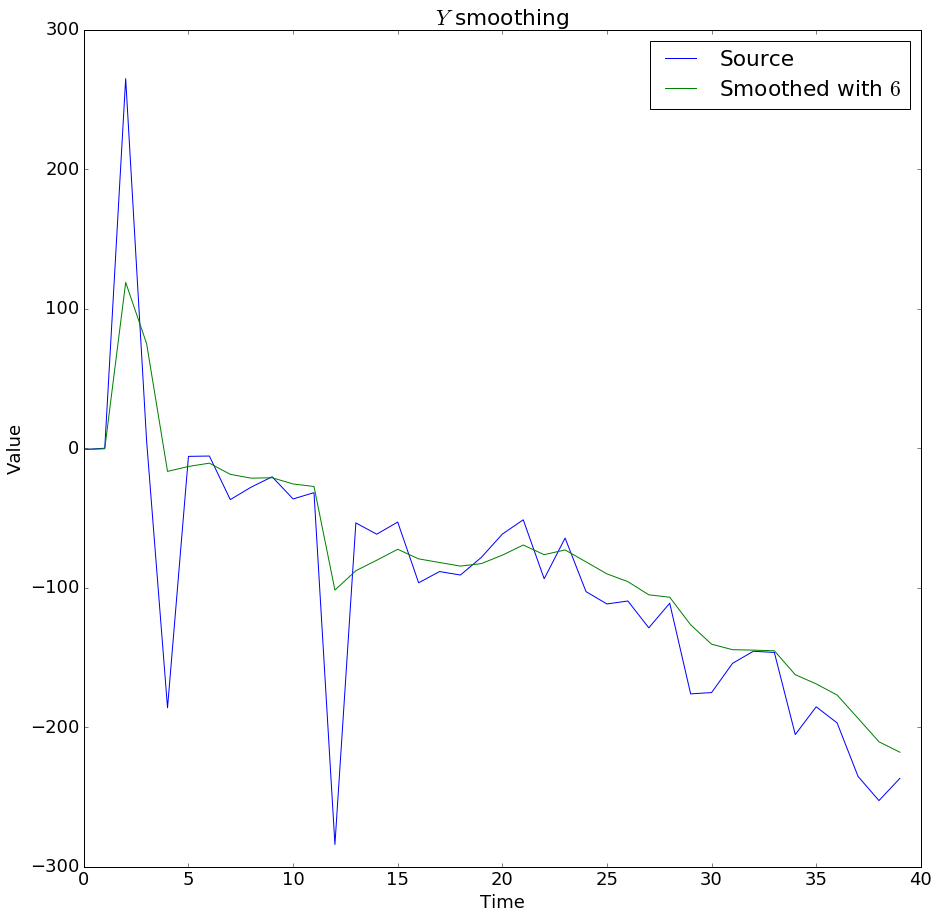
\includegraphics[width=\textwidth]{Coursework_files/Coursework_12_0.png}
  \caption{Зглажування ряду з аномаліями}
  \label{fig:anomaly:source}
\end{figure}

% \begin{center}
%   \adjustimage{max size={0.9\linewidth}{0.9\paperheight}}{Coursework_files/Coursework_12_0.png}
% \end{center}

Одразу видно, де знаходяться аномальні точки,
проте треба застосувати метод,
який ґрунтується на здоровому глузді
та математичній статистиці.
Оскільки аномальні точки заважають будувати лінію тренду,
потрібно порівняти якість фільтрації при видаленні різних точок даного ряду.
Введемо $Y_{fixed}\left( t \right)$ як ряд, в якому ``виправлено'' точку $t$.
Це означає, що дані в цій точці мають значення, яке не є аномальним.
Під якістю фільтрації розуміємо середньоквадратичне відхилення
між лінією тренду та самим рядом.
Порівняємо якість зглажування для $Y$
з якістю зглажування його виправленого аналогу.
Логічно, що можна порівняти їх співвідношення з певним граничним значенням
\begin{equation*}
  V\left( t \right)
  = \frac{Var\left( Y - Y^{smoothed} \right)}
         {Var\left( Y_{fixed}\left(t\right)
                    - Y_{fixed}^{smoothed}\left(t\right) \right)}
  > V_{critical}
\end{equation*}
Отримали вираз, що відомий як $F$-тест \cite{lomax2007statistical}:
маємо вибіркові дисперсії двох вибірок,
що за умовою мають нормальний закон розподілення.
Аномальні точки будемо знаходити одну за одною ---
знаходити найгіршу та виправляти її,
якщо вона дійсно аномальна
\begin{equation*}
  \max\limits_{t}{F_{F, T, T-1}\left( V\left( t \right) \right)}
    > F_{F, T, T-1}^{critical}
  \Longrightarrow
  t_{anomaly} = \max\limits_{t}{F_{F, T, T-1}\left( V\left( t \right) \right)}.
\end{equation*}
Поглянемо на те, як змінюється вибіркова дисперсія помилки
при відкиданні кожної точки на рис. \ref{fig:anomaly:variance}.
\begin{figure}[h!]
  \centering
  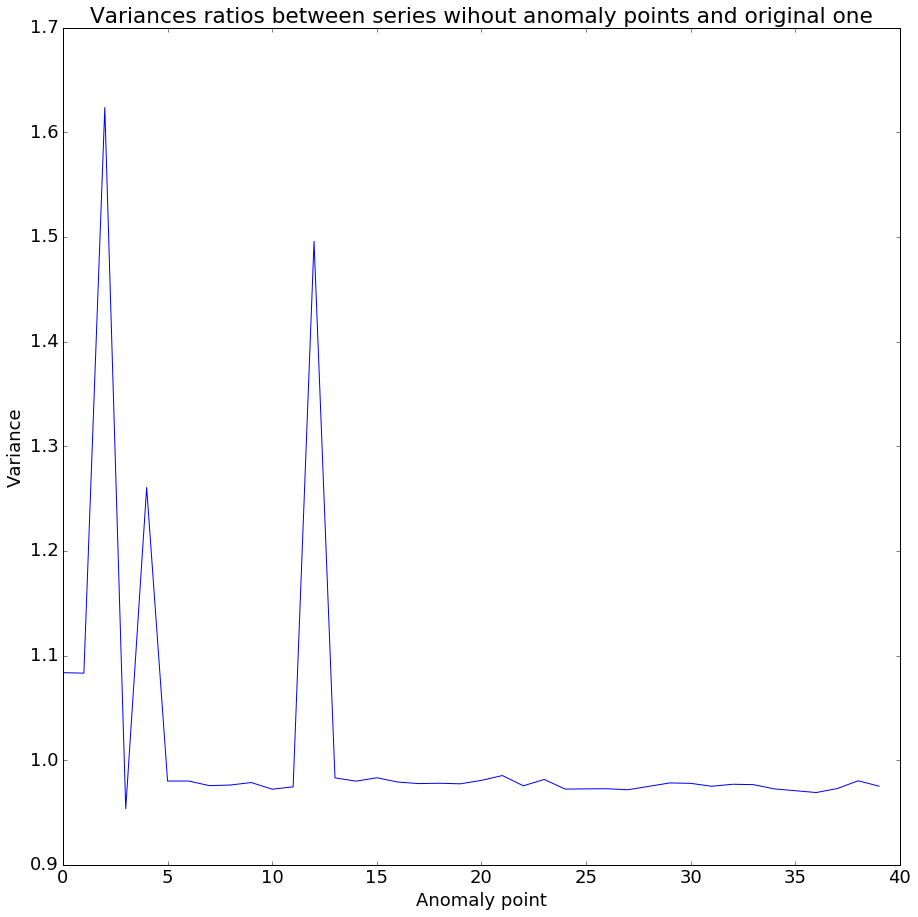
\includegraphics[width=\textwidth]{Coursework_files/Coursework_15_0.png}
  \caption{Відношення дисперсій помилок за виправлення певних точок}
  \label{fig:anomaly:variance}
\end{figure}

% \begin{center}
% \adjustimage{max size={0.9\linewidth}{0.9\paperheight}}{Coursework_files/Coursework_15_0.png}
% \end{center}

З рисунку видно піки саме в тих місцях,
де передбачалась наявнисть аномальних точок.
Проте зараз в нас є міра їх ``аномальності''
у вигляді ваги хвостів розподілу Фішера (рис. \ref{fig:anomaly:fisher}).
\begin{figure}[h!]
  \centering
  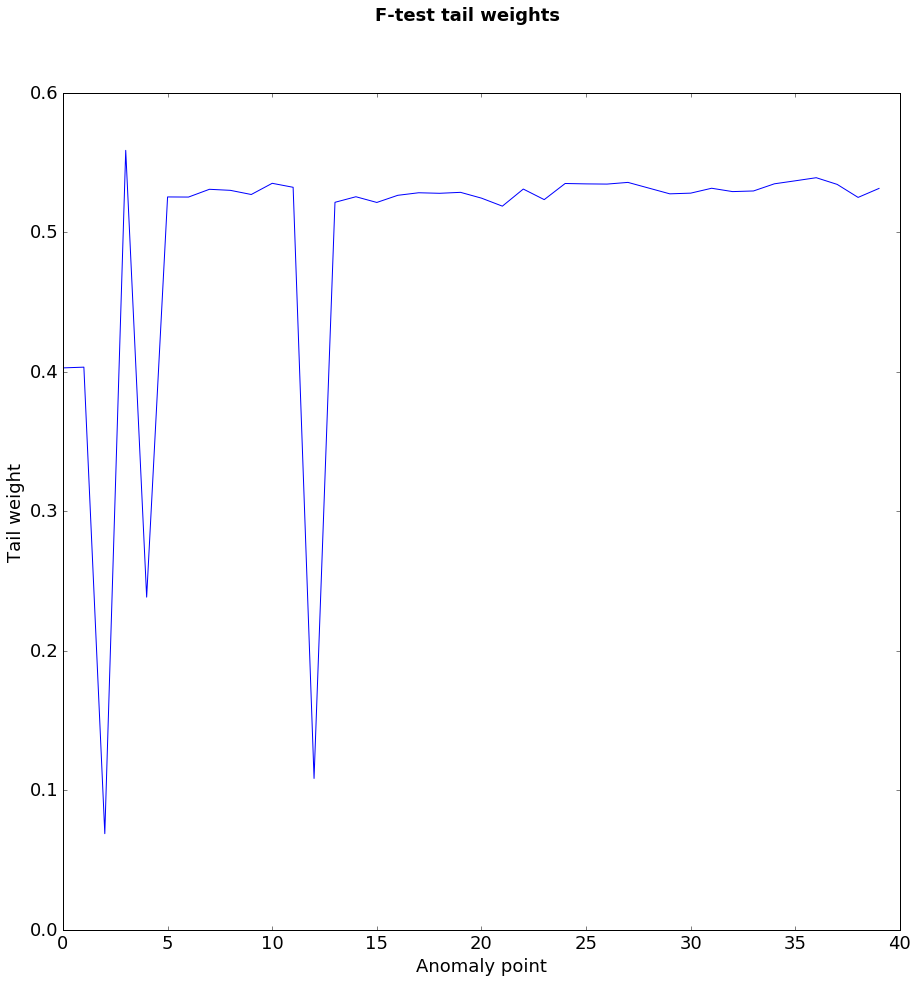
\includegraphics[width=\textwidth]{Coursework_files/Coursework_17_0.png}
  \caption{Хвости розподілу Фішера для відношень дисперсій виправлених рядів}
  \label{fig:anomaly:fisher}
\end{figure}

% \begin{center}
% \adjustimage{max size={0.9\linewidth}{0.9\paperheight}}{Coursework_files/Coursework_17_0.png}
% \end{center}

Відкидаємо одну за одною точки, при яких дисперсія значно змінюється,
а саме такі, що з ймовірністю $0.9$ це дисперсія іншої виборки
(рис. \ref{fig:anomaly:fisher:0}, \ref{fig:anomaly:fisher:1},
\ref{fig:anomaly:fisher:2}).
\begin{figure}[h!]
  \centering
  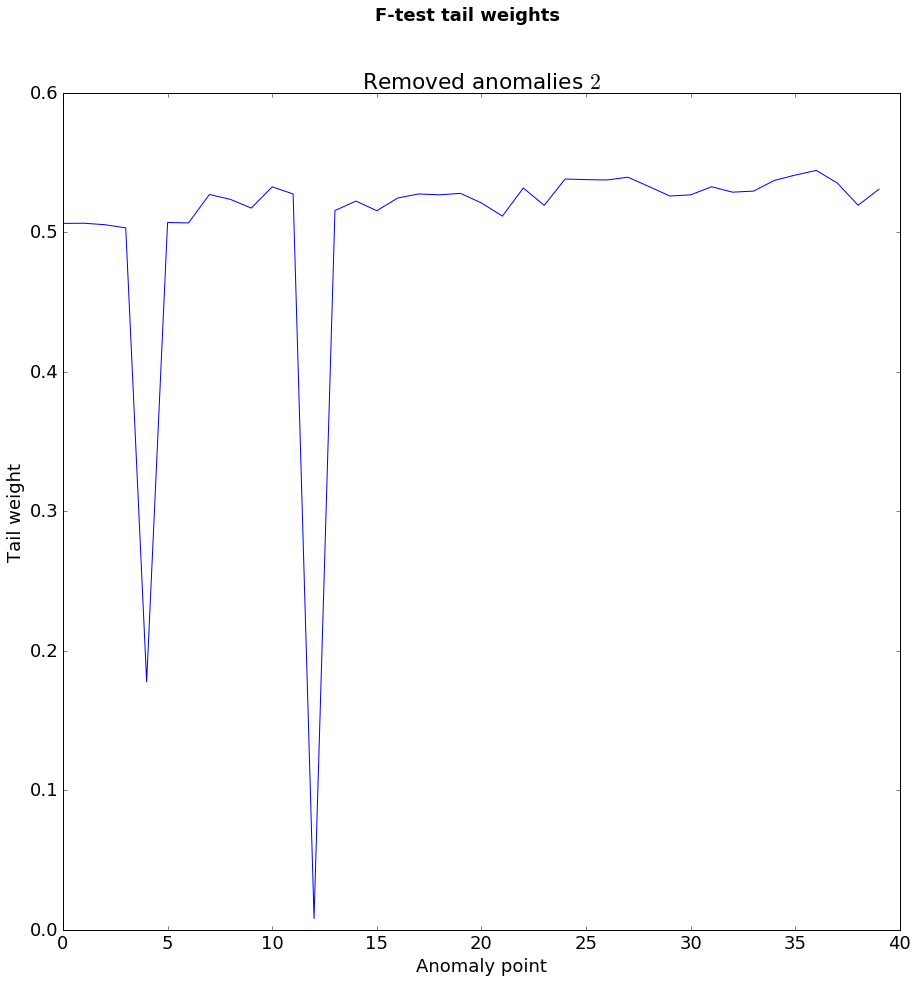
\includegraphics[width=\textwidth]{Coursework_files/Coursework_18_0.png}
  \caption{Хвости розподілу Фішера для відношень дисперсій виправлених рядів}
  \label{fig:anomaly:fisher:0}
\end{figure}
\begin{figure}[h!]
  \centering
  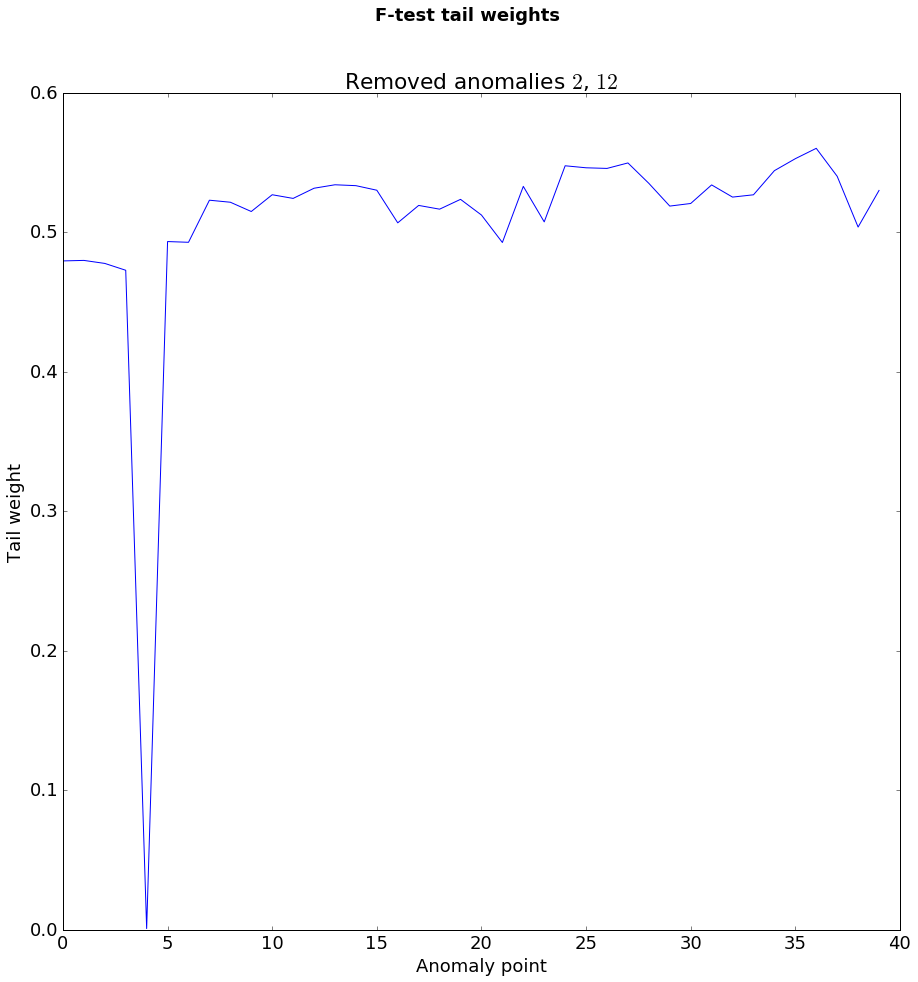
\includegraphics[width=\textwidth]{Coursework_files/Coursework_18_1.png}
  \caption{Хвости розподілу Фішера для відношень дисперсій виправлених рядів}
  \label{fig:anomaly:fisher:1}
\end{figure}
\begin{figure}[h!]
  \centering
  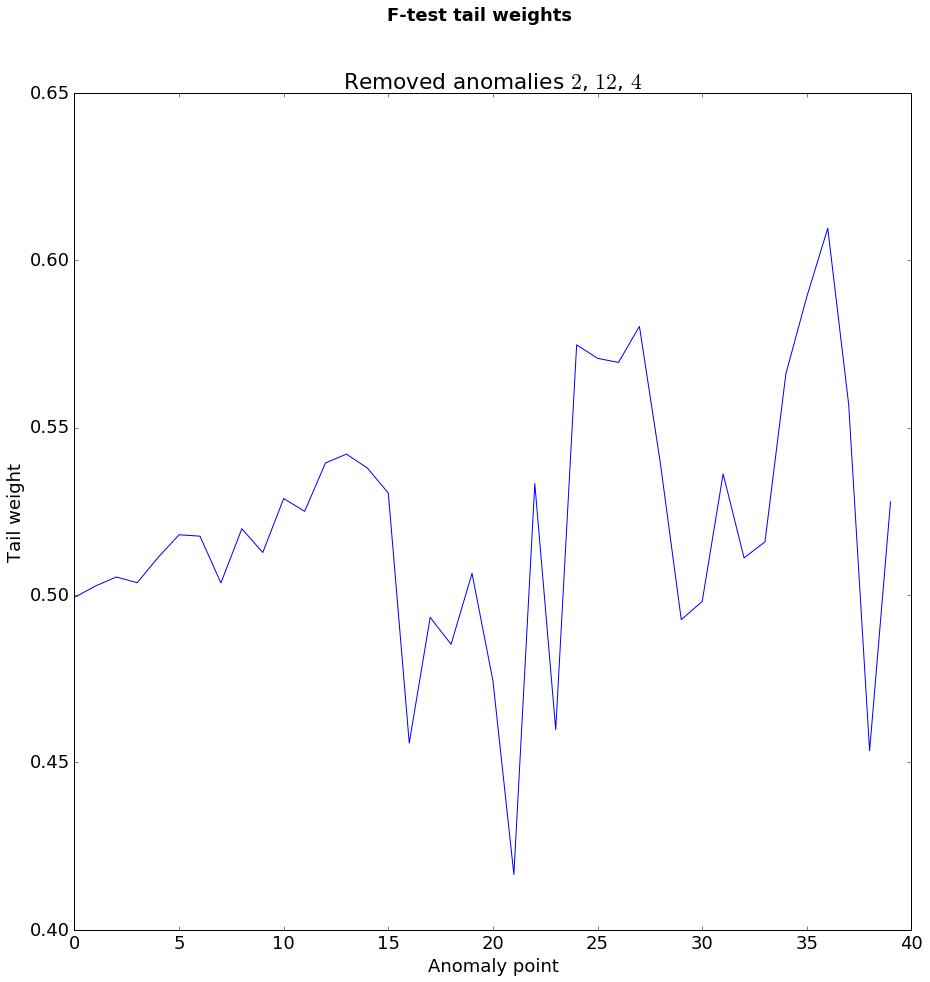
\includegraphics[width=\textwidth]{Coursework_files/Coursework_18_2.png}
  \caption{Хвости розподілу Фішера для відношень дисперсій виправлених рядів}
  \label{fig:anomaly:fisher:2}
\end{figure}

% \begin{center}
% \adjustimage{max size={0.9\linewidth}{0.9\paperheight}}{Coursework_files/Coursework_18_0.png}
% \end{center}
% 
% \begin{center}
% \adjustimage{max size={0.9\linewidth}{0.9\paperheight}}{Coursework_files/Coursework_18_1.png}
% \end{center}
% 
% \begin{center}
% \adjustimage{max size={0.9\linewidth}{0.9\paperheight}}{Coursework_files/Coursework_18_2.png}
% \end{center}

Аномальні дані знаходилися в точках $2$, $12$ і $4$.
Їх було виправлено за принципом найближчих сусідів ---
середнє арифметичне найближчих точок.
Маємо графік з даними без аномалій та зглажуванням,
яке тепер значно краще описує ряд

\begin{figure}[h!]
  \centering
  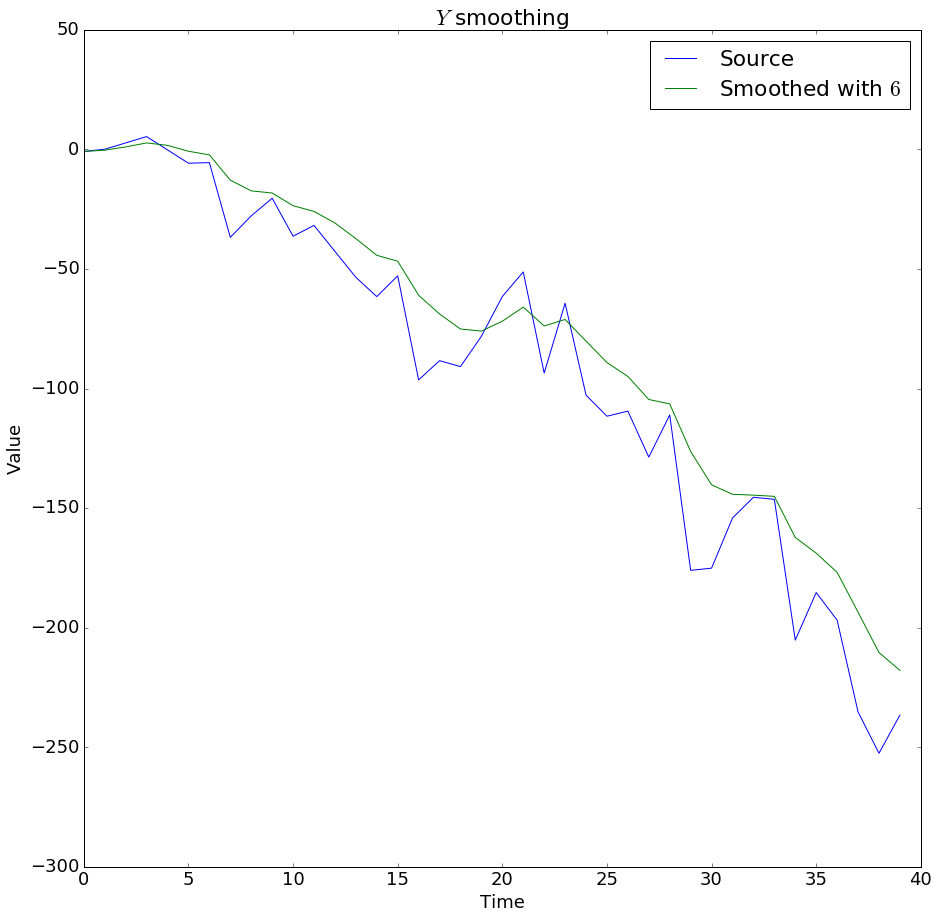
\includegraphics[width=\textwidth]{Coursework_files/Coursework_21_0.png}
  \caption{Оцінка виправленого ряду}
  \label{fig:anomaly:fixed}
\end{figure}
% \begin{center}
% \adjustimage{max size={0.9\linewidth}{0.9\paperheight}}{Coursework_files/Coursework_21_0.png}
% \end{center}

\section{Вибір правильного зглажуючого віконця}

Для подальших обчислень потрібно обрати коректні параметри зглажування,
а саме параметр $\alpha$ для експоненційно зглаженого ковзкого середнього.
Зазвичай це робиться в залежності від природи даних ---
їх циклічності або характерного часу зміни.
Цієї інформації немає, проте ми знаємо, що помилки мають гаусовий розподіл.
Скористуємося відомим методом
для визначення ``нормальності'' розподілу виборки ---
методом Д'Ауґустіно Ральфа \cite{dago1990}.
Цей тест на виході дає відстань розподілу даної виборки
до класу нормально розподілених виборок.
Ми хочемо обрати таке зглажування,
щоб розподіл помилок був якомого більш гаусовим.
Потрібно обрати таке $\alpha$,
для якого відстань між розподілом помилок та нормальним розподілом
була наймешною.
Ця умова винонується для віконця шириною $7$,
що відповідає $\alpha = \frac{1}{4}$.
Маємо похибку $\sigma = 16.3$ (рис. \ref{fig:span:fixed}).

\begin{figure}[h!]
  \centering
  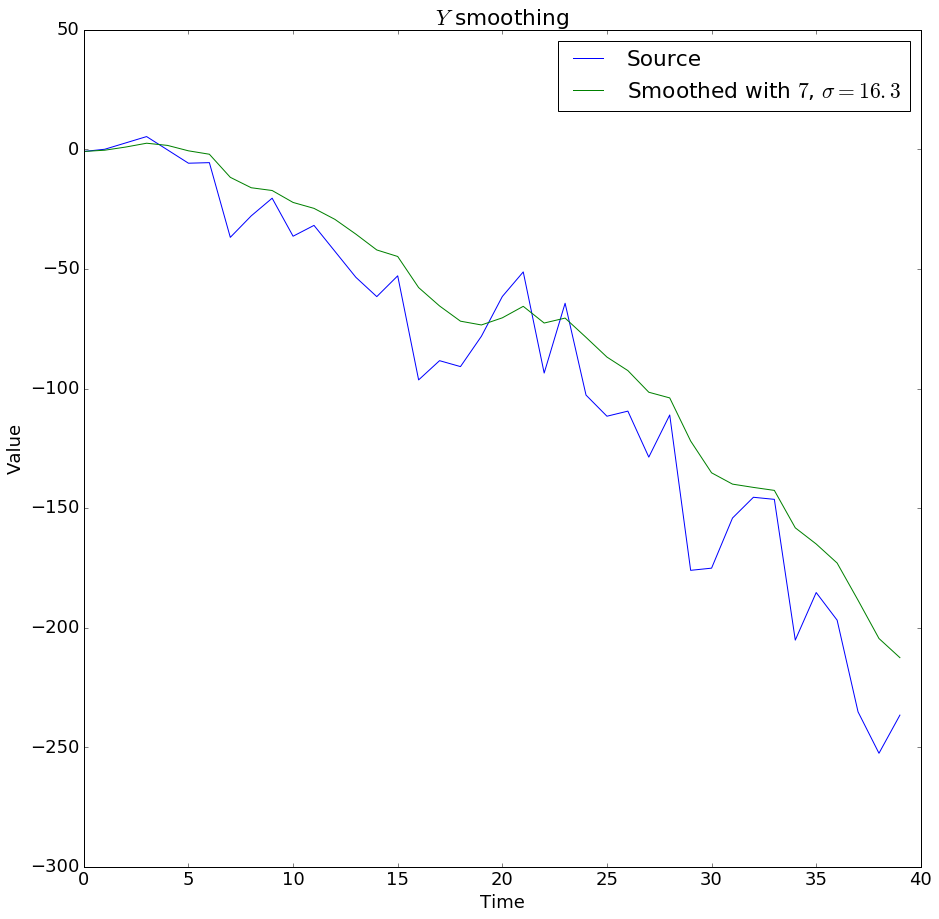
\includegraphics[width=\textwidth]{Coursework_files/Coursework_24_0.png}
  \caption{Помилки тренду}
  \label{fig:span:fixed}
\end{figure}
% \begin{center}
% \adjustimage{max size={0.9\linewidth}{0.9\paperheight}}{Coursework_files/Coursework_24_0.png}
% \end{center}

\section{Невипадкові похибки}

Лінія тренду може врахувати не всі закономірності ряду,
особливо якщо невідома його природа.
Наприклад, ми маємо ряд $Y$.
Позначимо його оцінку $\tilde{Y}$.
Тоді
\begin{equation*}
  \varepsilon = Y - \tilde{Y}.
\end{equation*}
Це призводить до того, що деякі помилки невипадкові,
тобто між ними є певна математична залежність.
Проаналізуємо простий випадок,
коли присутній деякий лаг $\tau$,
і помилки впливають не тільки на сусідні,
але й через певний час $\tau$.
Тоді помилка має випадкову $e$ та невипадкову частину $\delta$
\begin{equation*}
  \varepsilon_{t + \tau} = \delta_{t + \tau} + e_{t + \tau}.
\end{equation*}
Аналітичний вираз для невипадкової частини --- лінійна функція
\begin{equation}\label{nonrandom_error:eq}
  \delta_{t + \tau}
  = a_0 + \sum_{i = 0}^{\tau - 1} \delta_{t + i} \cdot a_{i + 1}.
\end{equation}
Дійсно видно, що середнє значення похибки ненульове,
тобто її можно як мінімум зсунути по вертикальній осі
(рис. \ref{fig:error:source}).
\begin{figure}[h!]
  \centering
  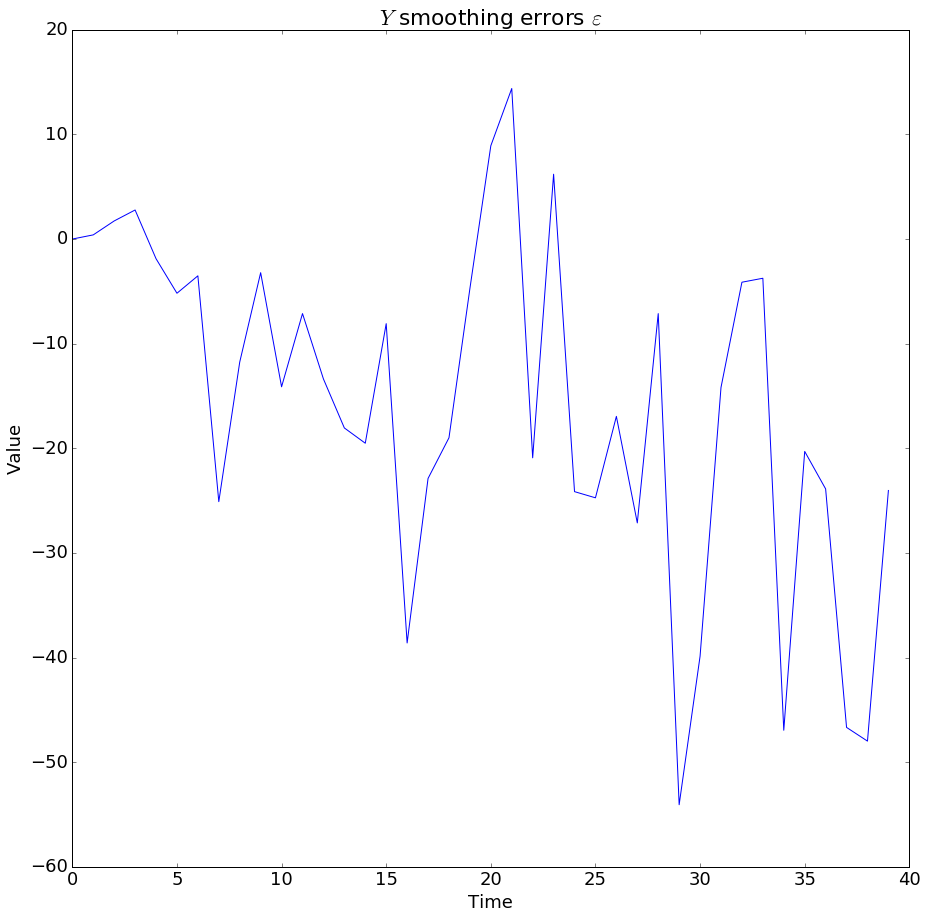
\includegraphics[width=\textwidth]{Coursework_files/Coursework_27_0.png}
  \caption{Фільтр з кращими параметрами}
  \label{fig:error:source}
\end{figure}
% \begin{center}
% \adjustimage{max size={0.9\linewidth}{0.9\paperheight}}{Coursework_files/Coursework_27_0.png}
% \end{center}

Щоб визначити величину лагу, потрібно порахувати авторегресії різних порядків.
Далі методом найменших квадратів розраховуються коефіцієнти для рівняння
\eqref{nonrandom_error:eq} (рис. \ref{fig:error:autocorrelation}).
\begin{figure}[h!]
  \centering
  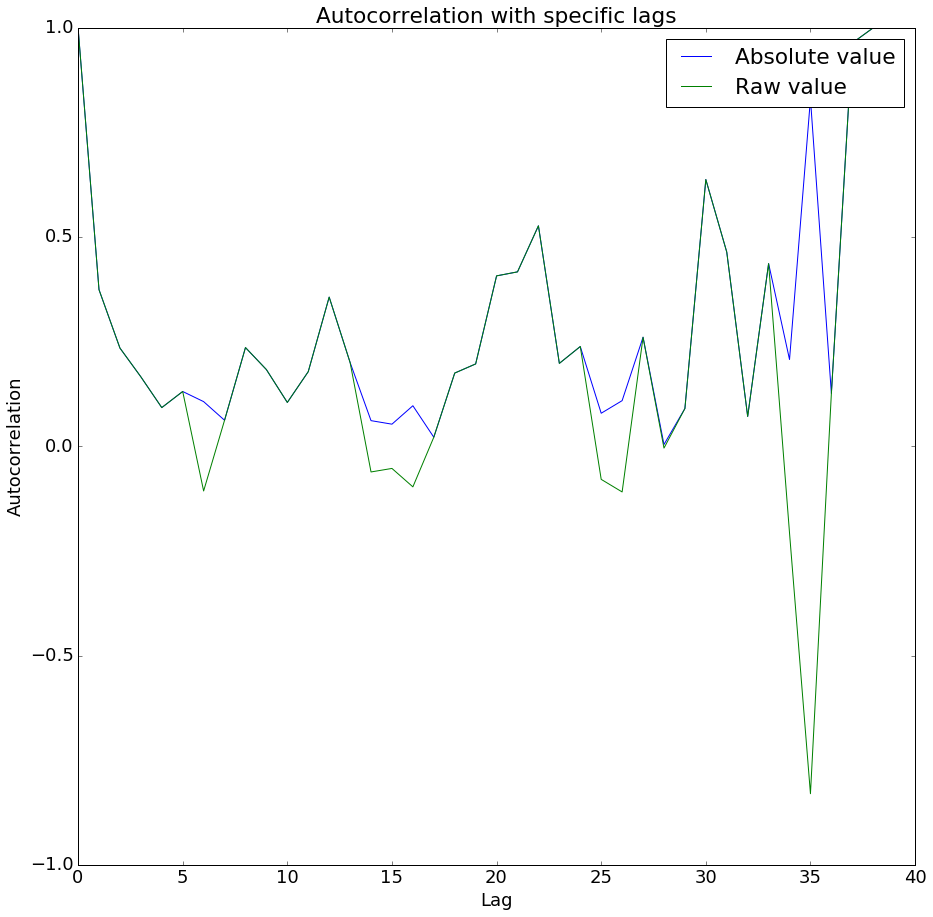
\includegraphics[width=\textwidth]{Coursework_files/Coursework_29_0.png}
  \caption{Автокореляція}
  \label{fig:error:autocorrelation}
\end{figure}
% \begin{center}
% \adjustimage{max size={0.9\linewidth}{0.9\paperheight}}{Coursework_files/Coursework_29_0.png}
% \end{center}

Обравши крок $2$, отримали хоч і невелику залежну частину,
проте помилка піднялась і тепер її середнє нульове.
Отримані коефіцієнти $a_i$: $0.12$, $0.31$, $-9.81$
(рис. \ref{fig:error:fixed}).
\begin{figure}[h!]
  \centering
  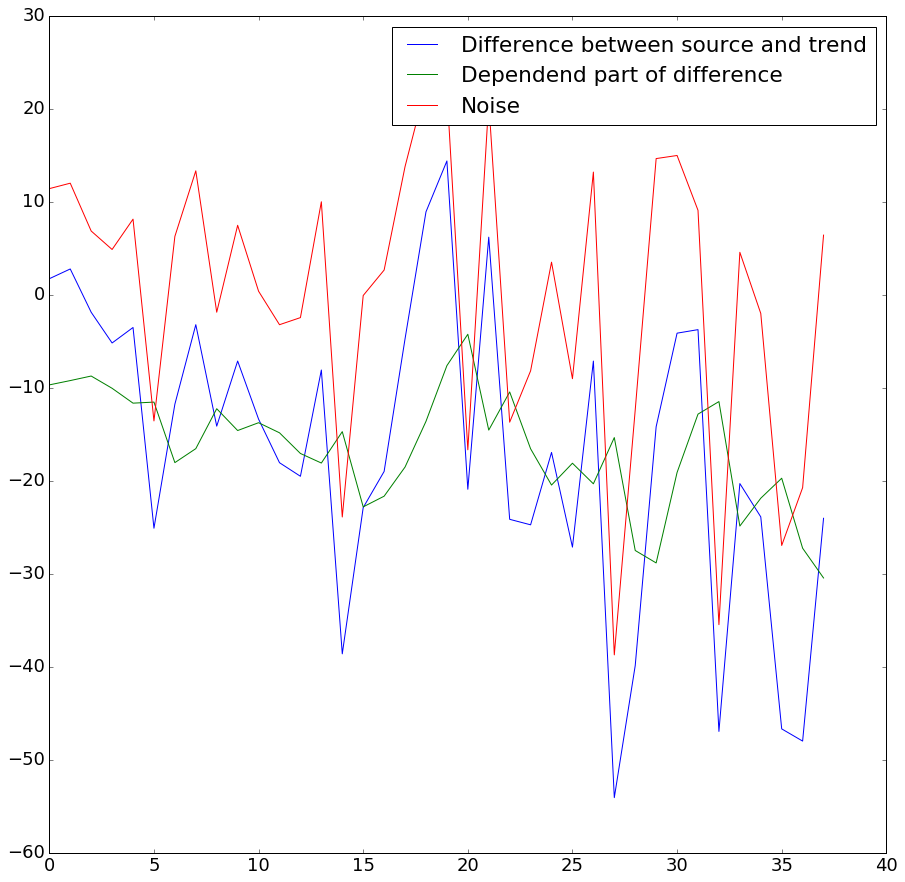
\includegraphics[width=\textwidth]{Coursework_files/Coursework_33_0.png}
  \caption{Порівняння помилки з оцінкою її невипадкової частини}
  \label{fig:error:fixed}
\end{figure}
% \begin{center}
% \adjustimage{max size={0.9\linewidth}{0.9\paperheight}}{Coursework_files/Coursework_33_0.png}
% \end{center}

Нова апроксимація ряду виглядає наступним чином та має меншу похибку
$\sigma = 15.1$ (рис. \ref{fig:error:estimate}).
\begin{figure}[h!]
  \centering
  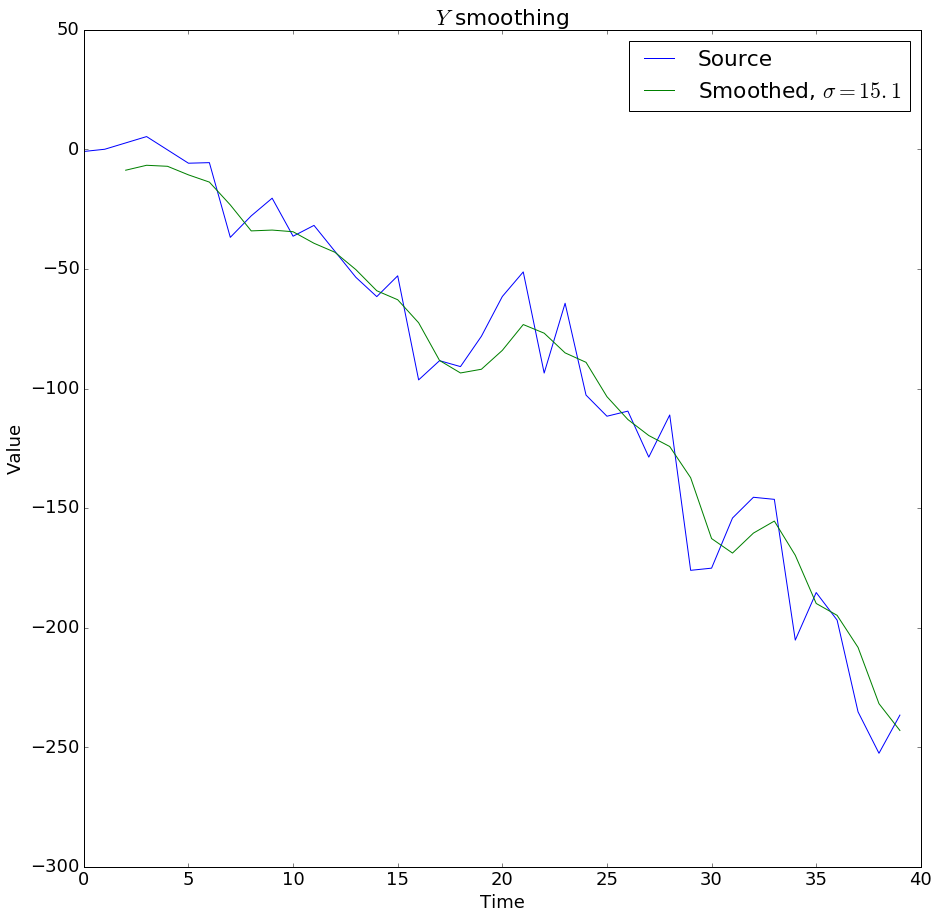
\includegraphics[width=\textwidth]{Coursework_files/Coursework_35_0.png}
  \caption{Апроксимація з урахуванням невипадкових помилок}
  \label{fig:error:estimate}
\end{figure}
% \begin{center}
% \adjustimage{max size={0.9\linewidth}{0.9\paperheight}}{Coursework_files/Coursework_35_0.png}
% \end{center}

\section{Прогнозування}

Наявна лінія тренду може бути спрогнозована за формулою
\begin{equation*}
  Y_{t + L} = \alpha_{0 t} + \alpha_{1 t} \cdot L + \frac{1}{2} \cdot \alpha_{2 t} \cdot L^2,
\end{equation*}
де
\begin{equation*}
  \begin{cases}
      \alpha_{0 t} = 3 \cdot \left( S_t^1 - S_t^2 \right) + S_t^3, \\
      \alpha_{1 t}
          = \frac{\alpha}{2 \cdot \beta^2} \cdot \left[
              \left( 6 - 5 \cdot \alpha \right) \cdot S_t^1
              - 2 \cdot \left( 5 - 4 \cdot \alpha \right) \cdot S_t^2
              + \left( 4 - 3 \cdot \alpha \right) \cdot S_t^3
            \right], \\
      \alpha_{2 t} = \frac{\alpha^2}{\beta^2} \cdot \left( S_t^1 - 2 \cdot S_t^2 \right) + S_t^3
  \end{cases}
\end{equation*}
і
\begin{equation*}
  \begin{cases}
      S_t^1 = \alpha \cdot Y_t + \beta \cdot S_{t-1}^1
            = \alpha \cdot \sum\limits_{i=0}^{t-1} \beta^i \cdot Y_{t-i} + \beta^t \cdot Y_0, \\
      S_t^2 = \alpha \cdot S_t^1 + \beta \cdot S_{t-1}^2, \\
      S_t^3 = \alpha \cdot S_t^2 + \beta \cdot S_{t-1}^3.
  \end{cases}
\end{equation*}
Проте нам вистачить лінійного прогнозу,
тому член формули з квадратом відкинемо
\begin{equation*}
  Y_{t + L} = \alpha_{0 t} + \alpha_{1 t} \cdot L.
\end{equation*}

Щоб приблизно визначити якість прогнозу,
можемо побудувати його для вже існуючих даних та порівняти
(рис. \ref{fig:forecast:initial}).
\begin{figure}[h!]
  \centering
  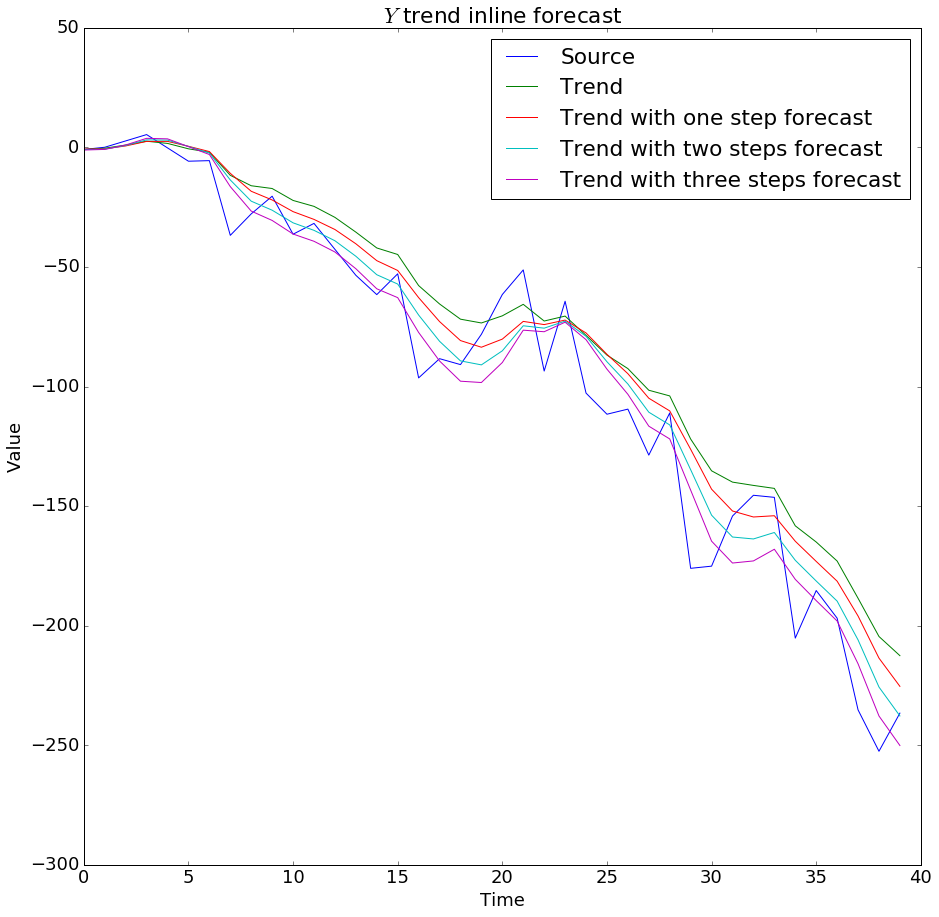
\includegraphics[width=\textwidth]{Coursework_files/Coursework_41_0.png}
  \caption{Прогнозування ретроданих}
  \label{fig:forecast:initial}
\end{figure}
% \begin{center}
% \adjustimage{max size={0.9\linewidth}{0.9\paperheight}}{Coursework_files/Coursework_41_0.png}
% \end{center}
Прогноз на три кроки після останньої точки має вигляд
(рис. \ref{fig:forecast:y}).
\begin{figure}[h!]
  \centering
  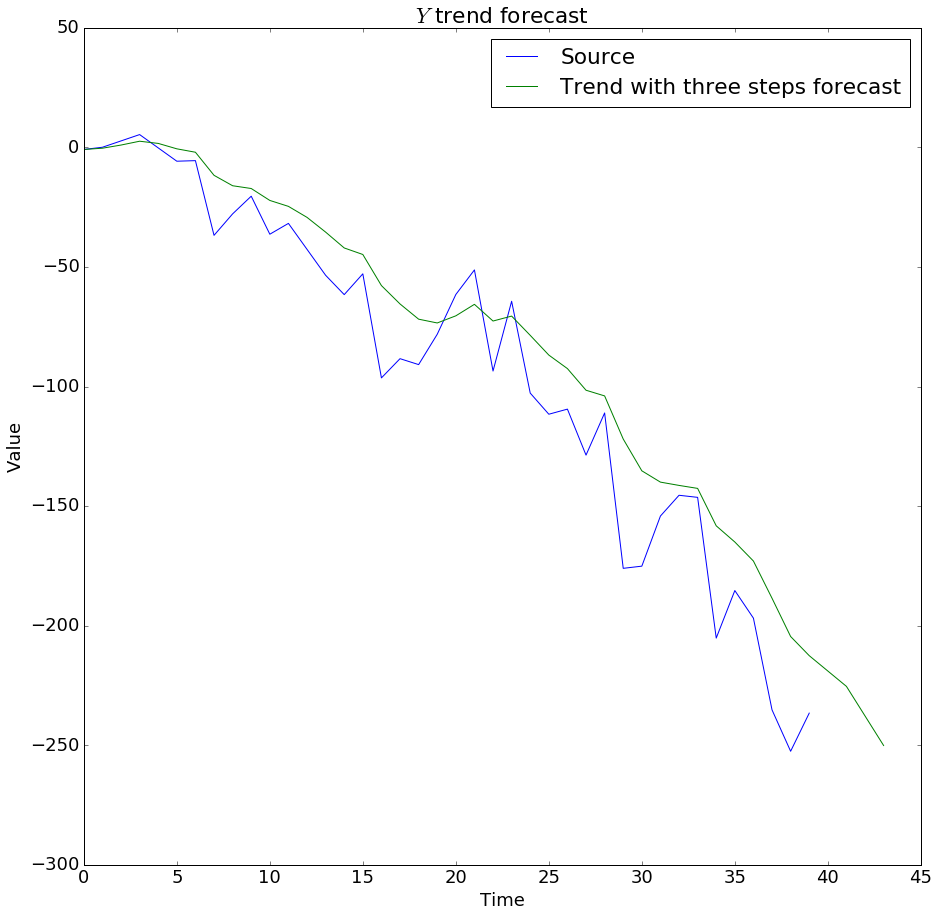
\includegraphics[width=\textwidth]{Coursework_files/Coursework_42_0.png}
  \caption{Прогноз}
  \label{fig:forecast:y}
\end{figure}
% \begin{center}
% \adjustimage{max size={0.9\linewidth}{0.9\paperheight}}{Coursework_files/Coursework_42_0.png}
% \end{center}

\section{Прогнозування невипадкових помилок}
Ми маємо лінійну формулу для розрахунку залежності
між невипадковими помилками
\begin{equation*}
  \delta_{t + 2} = a_0 + \delta_{t} \cdot a_1 + \delta_{t + 1} \cdot  a_2.
\end{equation*}
Перевіримо якість прогнозу у той самий спосіб ---
порівняємо його з наявними даними (рис. \ref{fig:forecast:errors}).
\begin{figure}[h!]
  \centering
  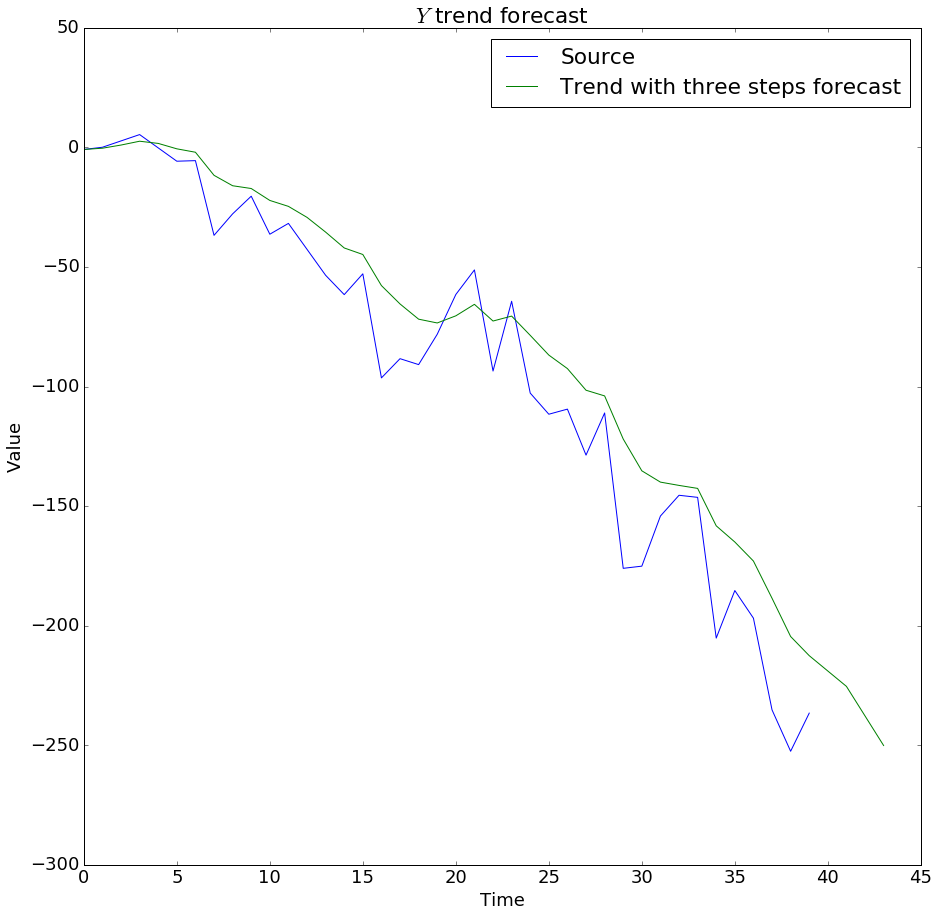
\includegraphics[width=\textwidth]{Coursework_files/Coursework_42_0.png}
  \caption{Прогнозування ретроданих з урахуванням невипадкових помилок}
  \label{fig:forecast:errors}
\end{figure}
% \begin{center}
% \adjustimage{max size={0.9\linewidth}{0.9\paperheight}}{Coursework_files/Coursework_44_0.png}
% \end{center}

\section{Прогноз процесу}
Кінцевий прогноз виглядає наступним чином
(рис. \ref{fig:forecast:with_errors}).
\begin{figure}[h!]
  \centering
  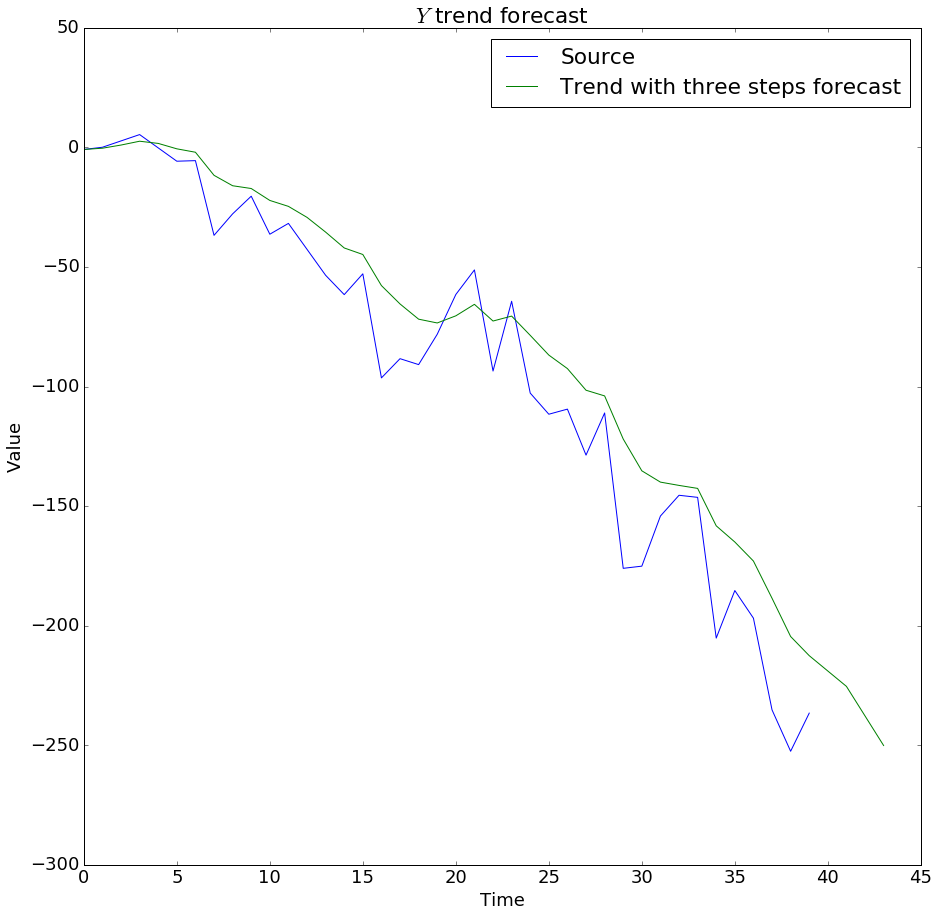
\includegraphics[width=\textwidth]{Coursework_files/Coursework_42_0.png}
  \caption{Прогноз з урахуванням невипадкових помилок}
  \label{fig:forecast:with_errors}
\end{figure}
% \begin{center}
% \adjustimage{max size={0.9\linewidth}{0.9\paperheight}}{Coursework_files/Coursework_47_0.png}
% \end{center}
